% a-project.tex, v-1.0.3 marcoreis baseado no
% abntex2-modelo-trabalho-academico.tex, v-1.9.7 laurocesar
% Copyright 2012-2018 by abnTeX2 group at http://www.abntex.net.br/ 
% 
% This work consists of the files ........
% 
% -----------------------------------------------------------------------------
% Modelo para desenvolvimento de documentação de projetos acadêmicos
% (tese de doutorado, dissertação de mestrado e trabalhos de monografias em geral) 
% em conformidade com ABNT NBR 14724:2011: Informação e documentação. 
% -----------------------------------------------------------------------------
% Opções para a documentação
%
% Fancy page headings 
%\documentclass[fancyheadings, subook]{Classes/a-prj}
%\documentclass[fancyheadings, sureport]{Classes/a-prj}
%
% Fancy chapters and sections headings 
%\documentclass[fancychapter, subook]{Classes/a-prj}
%\documentclass[fancychapter, sureport]{Classes/a-prj}
%
% Fancy page , chapters and sections headings
%\documentclass[fancyheadings, fancychapter, subook]{Classes/a-prj}
\documentclass[fancyheadings, fancychapter, sureport]{Classes/a-report}
%
% -----------------------------------------------------------------------------
% Alguns comandos para a fancy page headings)
%
% Page header line width
%\footlinewidth{value}
%
% Page footer line width
%\headlinewidth{value}
%
% Page header and footer line width
%\headingslinewidth{value}
%
% Page header and footer lines without text
%\headingslinesonly
%
% The default line width is 0.3pt.
% Set the value to 0pt to remove the page header and/or footer line
%
% -------------------------------------------------------------------------------
% Formato de figuras suportado
% -------------------------------------------------------------------------------
% O formato das figuras depende da forma como o arquivo de saída é gerado.
% As figuras inseridas na pasta Figures serão automaticamente reconhecidas sem
% a necessidade de inserir a extensão do arquivo.
%
% O pdfLaTEX (PDF) suporta figuras com as extensões: pdf, jpg, png e mps.
%
% -------------------------------------------------------------------------------
% Árvore do diretório a-project.tex
%  Diretório
%       \Classes        (requerido)
%       \Figures        (requerido) --------------------------------->
%       \Figures\PDF    (optional)
%       \Figures\JPG    (optional) Figures located within these
%       \Figures\PNG    (optional) folders are searched automatically
%       \Figures\MPS    (optional)  by the a-prj class.
%       \Figures\EPS    (optional)
%       \Figures\PS     (optional) <--------------------------------
%       \Tables         (requerido)
%       \Others         (requerido)
%       \Chapters       (requerido)
%       \Appendices     (optional)
%       \References     (requerido)
%
% -------------------------------------------------------------------------------
% PDF File resumo
\ifpdf
    \hypersetup{
    	backref,
        colorlinks  = true,
        pdftitle    = Modelo de documentação,
        pdfauthor   = {Marco Reis, marco.a.reis@gmail.com},
        pdfsubject  = Mestre em Engenharia,
        pdfcreator  = Subtitulo,
        pdfproducer = PDFLatex,
        pdfkeywords = {documentação, latex, dissertação, tese}}
 \fi
%
% -------------------------------------------------------------------------------
% Relação de pacotes opcionais utilizados
\usepackage[utf8]{inputenc}
\usepackage[brazil]{babel}
\usepackage{longtable}
\usepackage{dcolumn}
\usepackage{multirow}
\usepackage{lscape}
%\usepackage{graphicx}
\usepackage{rotating}
%\usepackage{float,subfigure}
%\usepackage{graphicx, subfigure}
\usepackage{cite}
\usepackage[left=3cm,top=3cm,right=2cm,bottom=2cm]{geometry}
\usepackage[alf]{abntex2cite}
\usepackage{ifpdf}
\usepackage{shadow}
\usepackage{wrapfig}
\usepackage[normalem]{ulem}
\usepackage{makeidx}
\usepackage{yfonts}
\usepackage{algorithm}
\usepackage{algorithmic}
\usepackage{lmodern}
\usepackage[T1]{fontenc}
\usepackage{indentfirst}
\usepackage{color}
\usepackage{microtype}
\usepackage{lipsum}
\usepackage{caption}
\usepackage{subcaption}
%
\makeindex 
\setlength{\LTcapwidth}{\textwidth}
%
\newtheorem{theorem}{Teorema}
\newtheorem{definition}[theorem]{Definição}
%
% -------------------------------------------------------------------------------
% Configurações do pacote backref
\renewcommand{\backrefpagesname}{Citado na(s) página(s):~}
% Texto padrão antes do número das páginas
\renewcommand{\backref}{}
% Define os textos da citação
\renewcommand*{\backrefalt}[4]{
	\ifcase #1 %
		Nenhuma citação no texto.%
	\or
		Citado na página #2.%
	\else
		Citado #1 vezes nas páginas #2.%
	\fi
}
% 
% -------------------------------------------------------------------------------
% Início do documento raiz
\begin{document}
% Definição do título da página
    \university{Centro Universitário SENAI CIMATEC}
	%\faculty{Programa de...}
	%\school{Escola de...}
% 
    %\course{Engenharia Elétrica}
    \typework{Relatório Final}
% 
	%\course{Mestrado em Modelagem Computacional e Tecnologia Industrial}
	%\typework{Disserta\c{c}\~ao de mestrado}
	%\typework{Exame de Qualificação de Mestrado}
% 
	%\course{Engenharia Elétrica}
	%\typework{Tese de doutorado}
	%\typework{Exame de Qualificação de doutorado}
%
% -------------------------------------------------------------------------------
% Informações gerais
    \thesistitle{Relatório Final das Ativades reazliadas no Centro de comptência de robótica e sistemas autônomos}
    \hidevolume
    \thesisvolume{Volume 1 of 1}
    \thesisauthor{Matheus Anselmo da Silva}
    
    \thesisadvisor{Prof. Marco Reis, M.Eng.}
    %\hidecoadvisor
    %\thesiscoadvisor{Marco Reis}
    \thesismonthyear{Agosto de 2022}
% 
    \maketitlepage
%
% ----------------------------------------------------------------------------
% Inserir Folha de rosto, Nota de estilo, folha de assinaturas, dedicatoria
    \include{Others/FolhaRosto}
    %\include{Others/NotaEstilo}
    %\include{Others/FolhaAssinaturas}
    %\include{Others/dedicatoria}
    %\include{Others/agradecimentos}
%
% ----------------------------------------------------------------------------
% Resumo/abstract, sumário e siglas
    \begin{romanpagenumbers}
        \begin{thesisresumo}
    Este relatório tem como objetivo apresentar os resultados na execução do programa de formação de pesquisadores  na área de robótica e sistemas de autônomos. As atividades desenvolvidas foram: aplicação e contextualização para de conceitos e de estaisticas, atividades com robôs manipula odres, elaboração de artigos e resumo estendidos, elaboração de linha de pesquisa voltada para robótica sub-aquática.

\ \\

% use de três a cinco palavras-chave

\textbf{Palavras-chave}: makeindex, Robótica Submarina, PManipuladores, Estaisticas, Palavra-chave 5

\end{thesisresumo}

        \begin{thesisabastract}
  
    This report aims to present the results in the execution of the training program for researchers in the area of robotics and autonomous systems. The activities developed were: application and contextualization of concepts and statistics, activities with robots to manipulate wineskins, elaboration of extended articles and abstracts, elaboration of a line of research focused on underwater robotics.
\ \\

% use de tr�s a cinco palavras-chave

\textbf{Keywords}: underwater robotics, Manipulators, statistics.

\end{thesisabastract}

        % Make list of contents, tables and figures
        \thesiscontents
        \pdfbookmark[1]{Lista de Tabelas}{lot} \listoftables
        \newpage
        %Include other required section
        %\include{Others/abbreviation}
        %\include{Others/simbolos}
        %Switch the page numbering back to the default format
    \end{romanpagenumbers}
%
% ---------------------------------------------------------------------------
% Include thesis chapters
    \parskip=\baselineskip
    \chapter{Introdução}
\label{chap:intro}

A dinâmica da socideade humanana sempre passou por mundanças em diveros aspectos:trabalho, social, ecônomico, politico, culutural e diveros outros. Nos ultimos anos, a presença de sistema com um certo grau de autonomia adiquiriu presença nas em diversas atividades que humanaas. Estas presenças acabam gerando influência de como o trabalho é visto e também na economia de diversas socideades.

evido ao crescimento de aplicações de robótica, e também, por algumas necessidaes que estão aparecento tanto para o ambiente residencal quanto industrial, há necessidade haver pessoas capacitadas para atuar na pesuisa e desenvolvimentos destas aplicações.

Durante o mês de Janeiro de 2022 até julho do mesmo ano, várias ativiaddes fora executadas no intuito de criar um base tanto na parte teorica quanto na prática para a formação de pesquisadores na área de robótica e sistemas autônomos.  As atividades foram: aplicação e contextualização para de conceitos e de estaisticas, atividades com robôs manipula odres, elaboração de artigos e resumo estendidos, elaboração de linha de pesquisa voltada para robótica sub-aquática.


%--------- NEW SECTION ----------------------
\section{Objetivos}
\label{sec:obj}
Apresnsenta os resultados alcançados no prgrama de formação de pesquisadores na área de robótica e sistemas autônomos.
\label{sec:obj}

\subsection{Objetivos Específicos}
\label{ssec:objesp}
Os objetivos específicos são:
\begin{itemize}
      \item Estudo de estaisticas.
      \item Estudo de robótica sub-aquática.;
      \item Elaboração de resumo estendido;
      \item Elaboração de artigos;
      \item Atividades com robôs manipula odres;
      \item Elaboração de linha de pesquisa voltada para robótica sub-aquática.
    
  \end{itemize}



%--------- NEW SECTION ----------------------
\section{Justificativa}
\label{sec:justi}

As atividades que encolvem sistemas autônoms estão crescendo quanto ao âmbito industrial e residencial. Novos robôs e novas soluções estão sendo desenvolvidas para estes ambiente.




%--------- NEW SECTION ----------------------
\section{Organização do documento}
\label{section:organizacao}

Este documento apresenta $5$ capítulos e está estruturado da seguinte forma:

\begin{itemize}

  \item \textbf{Capítulo \ref{chap:intro} - Introdução}: Contextualiza o âmbito, no qual a pesquisa proposta está inserida. Apresenta, portanto, a definição do problema, objetivos e justificativas da pesquisa e como este \thetypeworkthree está estruturado;
  \item \textbf{Capítulo \ref{chap:fundteor} - Fundamentação Teórica}: XXX;
  \item \textbf{Capítulo \ref{chap:metod} - Materiais e Métodos}: XXX;
  \item \textbf{Capítulo \ref{chap:result} - Resultados}: XXX;
  \item \textbf{Capítulo \ref{chap:conc} - Conclusão}: Apresenta as conclusóes, contribuições e algumas sugestões de atividades de pesquisa a serem desenvolvidas no futuro.

\end{itemize}

    \chapter{Conceito do projeto}
\label{chap:fundteor}
%--------- NEW SECTION ----------------------

Este capítulo tem  como foco apresentar os princinpais conceitos que envolvem o mercado de ROVs. Será apresentado a ambientalização do mercado de atuação dos ROVS e posteriomente a situação atual no desenvolvimento  destes veículos.
\section{Mercado de Atuação dos ROVs}



\section{Situação Atual do desenvolvimento}




%--------- NEW SECTION ----------------------


%---------------picture------------------------------------
% \begin{figure}
%     \centering
%     \subfigure[Figure A]{\label{fig:a}\includegraphics[width=60mm]{./lq}}
%     \subfigure[Figure B]{\label{fig:b}\includegraphics[width=60mm]{./lq}}
%     \subfigure[Figure C]{\label{fig:c}\includegraphics[width=\textwidth]{./lq}}
%     \caption{Three simple graphs}
%     \label{fig:three graphs}
% \end{figure}
%----------------------------------------------------------

% \begin{figure}
%     \centering
%     \begin{subfigure}[b]{0.3\textwidth}
%         \centering
%         \includegraphics[width=\textwidth]{./lq}
%         \caption{$y=x$}
%         \label{fig:y equals x}
%     \end{subfigure}
%     \hfill
%     \begin{subfigure}[b]{0.3\textwidth}
%         \centering
%         \includegraphics[width=\textwidth]{./lq}
%         \caption{$y=3sinx$}
%         \label{fig:three sin x}
%     \end{subfigure}
%     \hfill
%     \begin{subfigure}[b]{0.3\textwidth}
%         \centering
%         \includegraphics[width=\textwidth]{./lq}
%         \caption{$y=5/x$}
%         \label{fig:five over x}
%     \end{subfigure}
%        \caption{Three simple graphs}
%        \label{fig:three graphs}
% \end{figure}


% %--------- NEW SECTION ----------------------
% \section{Assunto 2}
% \label{sec:ass2}
% flkjasdlkfjasdlkfjs

% \begin{table}[h]
%     \begin{subtable}[h]{0.45\textwidth}
%         \centering
%         \begin{tabular}{l | l | l}
%         Day & Max Temp & Min Temp \\
%         \hline \hline
%         Mon & 20 & 13\\
%         Tue & 22 & 14\\
%         Wed & 23 & 12\\
%         Thurs & 25 & 13\\
%         Fri & 18 & 7\\
%         Sat & 15 & 13\\
%         Sun & 20 & 13
%        \end{tabular}
%        \caption{First Week}
%        \label{tab:week1}
%     \end{subtable}
%     \hfill
%     \begin{subtable}[h]{0.45\textwidth}
%         \centering
%         \begin{tabular}{l | l | l}
%         Day & Max Temp & Min Temp \\
%         \hline \hline
%         Mon & 17 & 11\\
%         Tue & 16 & 10\\
%         Wed & 14 & 8\\
%         Thurs & 12 & 5\\
%         Fri & 15 & 7\\
%         Sat & 16 & 12\\
%         Sun & 15 & 9
%         \end{tabular}
%         \caption{Second Week}
%         \label{tab:week2}
%      \end{subtable}
%      \caption{Max and min temps recorded in the first two weeks of July}
%      \label{tab:temps}
% \end{table}
    \chapter{Metodologia}
\label{chap:metod}
Nesta capitulo será descrito os procedimento, com os materias e métodos, para a realização do estudo do esuto da arte de ROVs que realizam ações de forma autonoma.

O metodo usado para alcançar o objetivo deste material foi o método BILI que consiste em executar uma busca otmizada de publicações sobre temas especificos.

\section{Metódo BilI}

O Método BiLi usa bibliotecas que estão presente na liguagem de progamação R,  a plataforma Mendely e a ferramenta cmpatools. A Figura \ref{fig:metodo_bili} demostra um fluxograma que representa a aplicação do Metodo Bili.  ANas próximas sessões serão apresentadas  cada etapa deste método.

%---------------picture------------------------------------
\begin{figure}
    \centering
   
    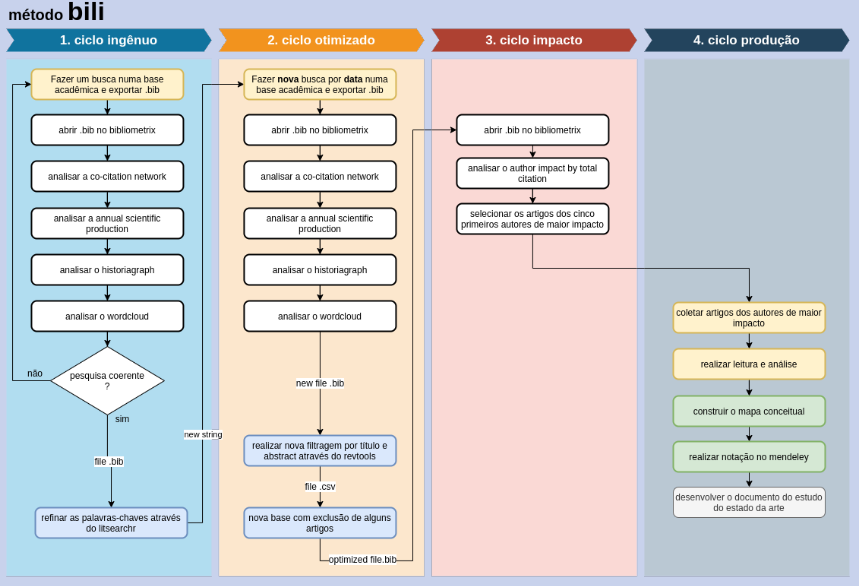
\includegraphics[width=\textwidth]{metodo_bili.png}
    \caption{Método Bili}
    \label{fig:metodo_bili}
\end{figure}
%----------------------------------------------------------
    \chapter{Revisão de Estaisticas}
\label{chap:stats}
Com objetivo de revisar e de aprender alugns conceitos importantes da estaistica, foi executado pequenas atividades usadando a linguagem de programação R. 
%escrever oq sera apresentado

\section{Principais conceitos que foram abordados}
Diveros conceitos foram aboradados e com o uso da lingaguem R, fora executadas algumas atividades que envolviam  aplicações de tecnicas de estaticas. os pricioais conceitos que foram aboradaos foram:
\begin{itemize}
\item Média, variância, e desvio padraão;
\item Distribuições;
\item Teste de Hipoteses;
\item Desgin de experimentos;
\item Análise de função de perda;
\item Análise de Pareto;
\item Análise de função de perda.

\end{itemize}

\section{Resultados}

A revisão de estaisticas foi bem sucedida. Além de reforçar os conhecimentos sobre estatiticas foi utilizado a linguem de programação. A importância desta revisão é importante, pois estes conceitos podem ser usados em na execuçãode projetos que envolva robótica e sistemas autônomas.



 
    \chapter{Resultados}
\label{chap:result}
Importante sempre ter um parágrafo introdutório para explicar os resultados encontrados.

%--------- NEW SECTION ----------------------
\section{Robôs Subaquáticos}

%Procurar algum artigo que possui definição de rovs
\label{underwater_robots}

De acordo com \cite{Bogue1}, Robôs Subaquáticos são importantes na exploração petroelo, militar e monitoramento de ambiente. Estes robôs são classificados em duas categorias diante ao modo de operação. Grande parte dos veículos dependem de intervenção humana, mesmo que mínima, para executar as funções.
A intervenção humana  acontece via teleoperação, comunamente por intermédio de um joystick. Estes robô são classificados como remotely operated vehicles (ROVs). Os veículos que não dependem de ações humanas, sistemas robóticos completamente autônomos, são os   Autonomous Underwater Vehicles (AUVs).

\subsection{Modelos de ROVs}

Existem vários modelos de robôs submarinos. O formato deste veículos podem ser em função de diversas considerações:local de atuação, profundidade onde as atividades serão executadas, suporte para a presença de braços manipuladores.

\subsubsection{BlueROV2}


O BlueROV2, representado na Figura \ref{fig:blue}, é desenvolvido pela Blue robotics, uma comphania americana especilizada em robô submarinos. Assim como informa \cite{Bluerobotics}, este veículo é destinado para realizar inpeções e pesquisas. O alcance de profundidade é de 100 m. 6 thursters são responsáveis pela atuação, 4 lâmpadas, também há versões com 6, e uma camêra HD coletar os dados visuais. 
Além destas configurações, outros intems pode ser adicionados ao exemplo de gripper, para realizar aconrragem, e sonares, para medição de profundidade e escananeamento. Um ponto importante do BlueROV2 é o fato de ROV ser opensource,  que permiti de várias modificações e dominio dos eventuais usuário.

\begin{figure}
  \centering 
  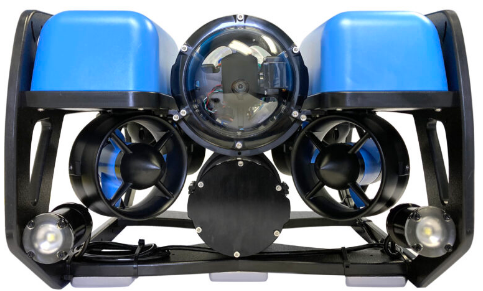
\includegraphics[width=150.5]{blue_rov.png}
  \caption{BlueROV2}
  \label{fig:blue}
\end{figure}

\subsubsection{Freedom ROV}


O Freedom ROV, apresentado na Figura \ref{fig:freedom_rov}, é desenvolvido pela comphania OCEANEERING, dentêm uma como a principal caracteristicas ter modos de operações híbridas. Segundo \cite{Bogue1}, Freedom pode operar sem intermédio de ações humanas, com ou sem a presença de cabos de comunicação. Este veiculo também capacidade de realizar \textit{subsea residence}, que é capacidade dos robôs ficarem alocadod no mar por um perido longo, neste caso seis meses. Durante o periodo de residência submarina, o Freedom ROV realizar o recarregamento de energia em estações de docagem submersas.


\begin{figure}
  \centering 
  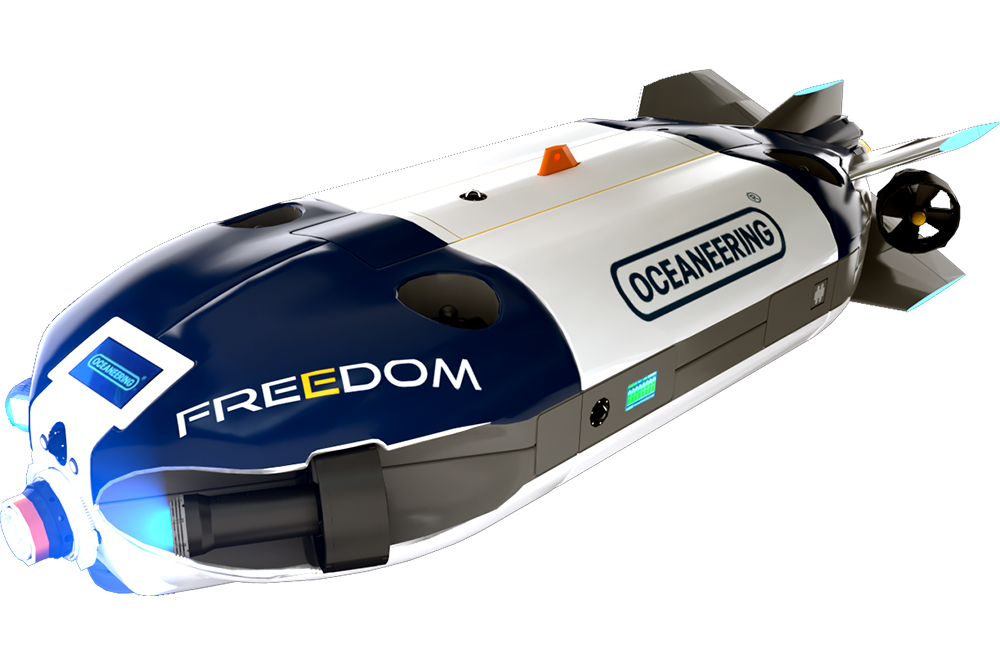
\includegraphics[width=150.5]{freedom_rov.png}
  \caption{Freedom ROV}
  \label{fig:freedom_rov}
\end{figure}

\subsubsection{SEASCAN MK2}


A ECA GROUP, uma companhia franceza especializada em desenvolver veículos marinhos e submarinos, desenvolveu um o ROV SEASCAN MK2, representado na Figura \ref{fig:seascan}. Este robô é tem uma forma de torpedo. De acordo com \cite{ECA_GROUP}, O SEASCAN é um veículo leve e pode ser usado para inspeções, identificação de minas e para missões com fins ambientais. Cabos umbilicais não são usados para nem para cominicação e nem para alimentação.  Uma bateria recarragável é a fonte de alimentação deste robô.

Também é apontado por \cite{ECA_GROUP} que o SEASCAN MK2 também pode realizar algumas duas tarefas autônomas. Uma é dedicada para realizar posicionamento diante a profundidade do veículo, a outra é focada em automatizar o caminho do veículo a alcançar uma area específica.



\begin{figure}
  \centering 
  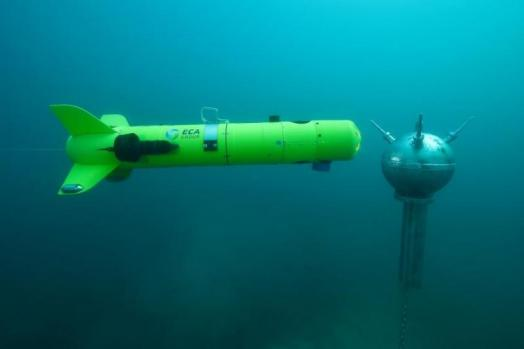
\includegraphics[width=150.5]{seascan.jpg}
  \caption{SEASCAN MK2}
  \label{fig:seascan}
\end{figure}


\subsubsection{Aquanaut ROV}

O Aquanaut ROV um é veículo, de acordo \cite{Bogue1}, que além de possuir operação hibrida, autonomo e teleoperado., também não possui um formato único. O Aquant ROV possui dois formatos de operação, um para o modo autonomo, e outro para realizar teleoperação.
A Figura \ref{aquanaut_auv} representa o Aquant na forma autonoma e  a Figura \ref{aquanaut_rov} é o foramto que o Aquant adiquiri ao passar para a atuação teleoperado.

O modo de atuação autonoma é realizada até o robô antingir o momento de realizar as atividades destinadas ao trabalhos com manipuladores. Para atuar de forma com os manipuladores, o Aquanaut mudar de formato e sua atuação passar a ser completamente por fins de teleoperação, em outras palavras há uma necessidade de presenaça  humana na operação. 


\begin{figure}
  \centering 
  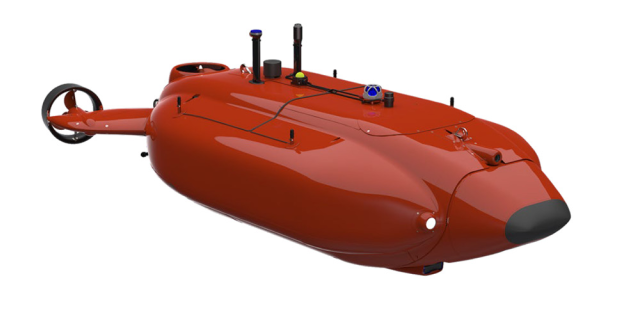
\includegraphics[width=150.5]{aquanaut_auv.png}
  \caption{Aquanaut em formato para realizar operações autonomanas}
  \label{fig:aquanaut_auv}
\end{figure}

\begin{figure}
  \centering 
  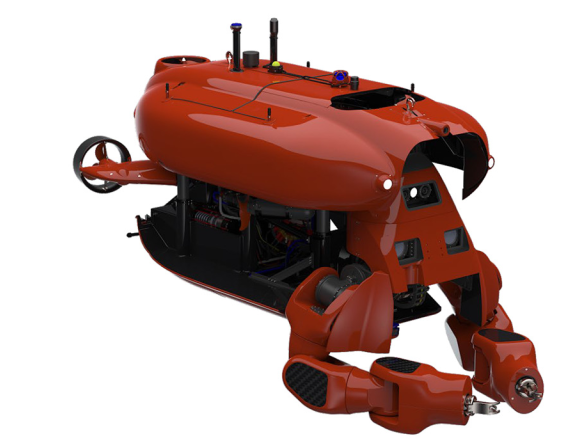
\includegraphics[width=150.5]{aquanaut_rov.png}
  \caption{Aquant em formato para teleoperação}
  \label{fig:aquanaut_rov}
\end{figure}



\subsection{Considerações na Modelagem}
Esta seção aborda os princiapis elementos e considerações para modelagens de ROVs.

Assim como quase todos robôs móveis podem estar posicionado em relação a uma referência, a posição de um robô subaquatico pode ser representando, de acordo com \cite{Antonelli}, diante a sua posição e orientação.
Diante a um Frame fixo de referência, é possivel obter a posição, usando técnicas de sensoriamentom, de um veículo submerso que comunalmente representando como vetor.
%vetor = (x,y,z)

Para representar a rotação dos veiculos diante ao mesmo frame pode usar o vetor
%n =(r,p,y)
que é a representação de roll, pitch  e yaw.

A seguinte tabela apresenta os movimentos dos veículos Subaquáticos em relação ao destes. Esta tabela esta de acordo que demostrado em \cite[Antonelli]. Estes movimentos, surge, sway e heave, também são usados navegações marinhas. Para acompanhar os movimentos dos ROVs sensores são comunalmente implementados nas estruturas destes.





%lembre de usar o livro de fossen
\subsection{Sensores}

A presença de sensores em um sistema pode permiti a obtenção de dados de vários. A medida dos sensores podem ser direcionados para a propria dinânica de um sistema, neste caso um ROV, e o ambinete no qual este realizar suas ações.
Assim como classifica \cite{Towards}, os sensores de um ROV pode distinguindo em dois grupos: \textit{playload sensors}  e \textit{navigations sensor}. Os \textit{payload sensors} são unidades de medidas destinados a coletar dados do ambiente, alguns exemplos destes sensores saão: sensores CTD, destinados a mensurar a condutividades, temperatura e profundidade, sensores ADCP-Acoustic Doppler Curent pPofiler- são usados para mensurar a velocidade das correntes e câmeras para obter dados visuais.

Os navigations sensors são implementados com o foco na navegação do veículo, logos dados sobre a posição, orientantçã e veocidade são os principais alvos a serem mensurados. Os navigations sensors mais comum são: sensores de pressão, (DVL) mede o deslocamento Doppler no sinal de entrada refletido no fundo do mar para obter os dados da velocidade linear e sensores de inercia. 
Câmeras também podem ser usadas para obter dados da posiação de veículos, assim como foi demostrado por \cite{visual_serving}, no qual foi ultizado duas câmeras par realizar um acomphamento da posição de ROV. Os dados dos sensores podem ser usados para o monitoramento e para as ações de controle.

% Colocar a tabela com as imagens dos principais sensores



\subsection{Controle}
% tipo de controle
Para os ROVs, grande parte do objetivo do contole é focado na movimentação. A aplicação de controle linear 
% objetivo de controle

\subsection{Atuação}
% Thrusters
%% Tipo de Thrusters
%Fins
% Tipos de Fins

\subsection{Arquitetura de Operação}
Há diversas formas que as arquiteturas de operação diante do nível de autonomia dos ROVs podem ser implementados. Uma comum é quando um humano é responsável 100\% das atuações do veículos, em outras palavras, é aplicado um controle 100\% manual. O operador, neste caso costuma ser um bastante habilidoso, comunalmente usa uma video câmera para estimar a posiação do veículo no ambiente.

% achar uma referência para o controle manual.

Uma arquitetura, segundo \cite{wireless_joy}, é \textit{Human in the Loop} - HITL- que é realizado considerando a arquitetura \textit{Human Centered Automantion} - HCA. Nesta arquitetura o operador humano realizar algumas tarefas do sistema de controle, ao exemplo de selecionar de qual mode de ação de movimento o veiculo deve realizar. Alguns exemplos dos modo de ação o controle de profundidade, heading e seguir tubulações.

Outros tipos de operações são apontadas por \cite{Towards}: \textit{Automatic Operation}, \textit{Management by consent}, \textit{Semi-autonomous or management by exception} e \textit{Highly autonomous}. O primeiro, \textit{Automatic Operation}, possui caracteristicas semelhante ao \textit{human in the loop} e o segundo, \textit{Management by consent} é basicamente uma teleoperação. O \textit{Semi-autonomous or management by exception} é montado para o sistema executar automaticamente as funções relacionadas à missão quando os tempos de resposta são muito curtos para intervenção humana.  Quando não necessidade de um operador realizar nenhuma intervenção sobre o veiculo, o tipo de operação é considerada \textit{Highly autonomous}. Esta última classificação esta mais proxima das condicções necessarios para um veículo submarino ser considerado um AUV. As estruturas de operação podem variar em função das atividades que os ROVs realizam e também considera os modelos destes. 








%--------- NEW SECTION ----------------------


\section{Revisão bibliográfica}
\subsection{Rede de Citação}
\subsection{Principais autores}

%--------- NEW SECTION ----------------------

\section{Mapa COnceitual}
\lipsum[1]

%--------- NEW SECTION ----------------------







    \include{Chapters/conclusao}
    % include more chapters ...
%
% ----------------------------------------------------------------------------
% Include thesis appendices
    \begin{thesisappendices}
        \include{Appendices/diagmec}
        \include{Appendices/diagele}
        %\include{Appendices/logbook}
    \end{thesisappendices}
%
% ----------------------------------------------------------------------------
% Configurar as referencias bibliograficas
	\renewcommand\bibname{Referências}
    \addcontentsline{toc}{chapter}{Referências}
    \bibliography{References/referencias}
%
% ----------------------------------------------------------------------------
% Finishing him
    \include{Others/ultimafolha}
\end{document}
%
% -------------------------------------------------------------------------------
% Aqui termina a formatação para o documento.
% In God We Trust. All Other Bring Data. 
%
% -------------------------------------------------------------------------------